\setcounter{chapter}{3}
\chapter{Contribution and Research Activities}

%******************** START Contribution and Research Activities. ***************
In this chapter we will introduce the important notions in argumentation-based negotiation,  
\section{Argumentation System and Agent Theory}\label{sec:Argumentation}
Let us recall some basic definitions in the argumentation-based negotiation.

\begin{definition}{\emph{[Move].}} \label{Move}
Let $Ag = \{Ag_1,Ag_2, \ldots\}$ be a set of symbols representing agent names that may be involved in a negotiation dialogue $D$. A
move $M_i\in D$ consists of the agent that utters the move: $Speaker(M_i)\in Ag$; the set of agents to which the move is
addressed: $Hearer(M_i)\subseteq Ag$; and the content of the move: $Content(M_i)$.
\end{definition}

For simplification reasons, we will consider bilateral negotiation (i.e., only two agents involved in the dialogue $Ag_1$ and $Ag_2$).
Multi-party dialogues is an important issue that we plan to investigate in future work. During a dialogue, several moves may be uttered.
Those moves constitute a dialogue $D$, which is a sequence of moves denoted by $[M_0$,$M_1$,\ldots,$M_n]$, where $M_0$ is the initial move,
$M_n$ is the final one, and $|D|$ is the length of the dialogue (i.e., $|D| = |[M_0$,$M_1$,\ldots,$M_n]| = n+1$).

In what follows, we assume that the agents exchange the content of the moves during the dialogue as arguments because our approach is
argumentation-based. In argumentation systems the logical language $\pounds$ is essential, we will recall the definition of the
argument concept, a definition of the attack relation between arguments, and the definition of acceptability
from~\cite{Amgoud00}, then we will use these definitions in our approach. Here $\Gamma$ indicates a possibly inconsistent
knowledge base with no deductive closure, and $\vdash$ stands for classical inference.

\begin{definition}{\emph{[Argument].}} \label{Argument}
An argument $Arg$ is a pair $(H, h)$ where $h$ is a formula of $\pounds$ and $H$ a subset of  $\Gamma$ such that: i) $H$ is
consistent, ii) $H \vdash h$ and iii) $H$ is minimal, so that no subset of $H$ satisfying both i and ii exists. $H$ is called the
support of the argument and $h$ its conclusion.
\end{definition}


\begin{definition}{\emph{[Attack].}} \label{Attack}
Let $(H, h)$, $(H^{\prime}, h^{\prime})$ be two arguments. $(H^{\prime}, h^{\prime})$ attacks $(H, h)$ iff $H^{\prime} \vdash
\neg h$. In other words, an argument is attacked iff there is an argument for the negation of its conclusion.
\end{definition}

Our dialogue architecture also involves general knowledge, such as knowledge about the dialogue subject. Agents can also reason about
their preferences in relation to beliefs. The idea is to capture the fact that some facts are believed more than others. For this
reason, we assume, like in~\cite{Mbarki06}, that any set of facts has a preference order over it. We suppose that this ordering
derives from the fact that the agent's knowledge base ($\Gamma$) is stratified into non-overlapping sets $\Gamma_1,\cdots ,
\Gamma_n$ such that facts in $\Gamma_i$ are all equally preferred and are more preferred than those in $\Gamma_j$ where $i < j$. The
preference level of a subset of $\Gamma$ whose elements belong to different non-overlapping sets is defined as follows.

\begin{definition}{\emph{[Preference Level].}} \label{preferenceLevel}
The preference level of a nonempty subset $\gamma$ of $\Gamma$ denoted by level $(\gamma)$ is the number of the highest numbered
layer which has a member in $\gamma$.
\end{definition}
\begin{example}
Let $\Gamma = \Gamma_1 \bigcup \Gamma_2 $ with $\Gamma_1$ = $\{ a, b\}$ and $\Gamma_2$ = $\{ c,d \}$ and $\gamma = \{a\}$ and
$\gamma\prime = \{a,d\}$. We have: level$(\gamma) = 1$ and level$(\gamma\prime) = 2$.
\end{example}

\subsection{Strategic and Tactic Reasoning}\label{sec:reasoning}
A preliminary framework for strategic and tactic reasoning for agent communication was proposed in~\cite{Mbarki06}. This
reasoning framework is specified using argumentation theory combined to a relevance theory. Strategic reasoning enables agents
to decide about the global communication plan in terms of the macro-actions to perform in order to achieve the main dialogue
goal. Tactic reasoning, on the other hand, allows agents to locally select, at each dialogue step the most appropriate
argument according to the adopted strategy.

In this paper, we refine, and use the notion of strategic and tactic reasoning. The agent uses his tactic reasoning at each dialogue
step to measure his uncertainty about selecting the right move to achieve some sub goals of the global goal (i.e., the agreement in our case).
In other words, how agent can select the right argument from a set of possible choices at certain dialogue step depends on his tactic by assigning
different probability values to the different arguments and select the one with higher probability to be accepted by his opponent. On the other hand,
this tactic is based on the adapted strategy that the agent built before starting the negotiation to achieve the agreement. Moreover, we study the
relationship between these two types of uncertainty not only when a unique move is considered, but also when the whole dialogue is being analyzed.


%\subsubsection{Strategic Reasoning}\label{sec:Strategic}
\textbf{Strategic Reasoning}\\
Before engaging in a negotiation, agents must build a global strategy on the sub-goals to achieve. Sub-goals determine the general steps to follow so
that the global goal can be realized. Strategy is subject to the agent's current beliefs and constraints, such as the agent's budget and negotiation
time limit. To achieve the same negotiation goal, an agent can have several alternative strategies reflected by different sets of subgoals. The dialogue
goal, sub-goals, and constraints can be expressed using propositional logic. The set of constraints can be inconsistent, but the sub-set of those constraints
and the sub-set of beliefs the agent decides to consider should be consistent. We define the strategy as a function that associates to a goal and a sub-set
of consistent beliefs and constraints a sub-set of alternatives, each of which is a set of sub goals, which means an element of the set $2^{2^{\mathbb{B}}}$,
where $\mathbb{B}$ is the set of goals.

\begin{definition}{\emph{[Strategy]\footnote{This definition is different than the one proposed in~\cite{Mbarki06}, in the sense that this function
associates a set of sub-goals to a sub-set of agent's knowledge base and constraints instead of associating a set of goals to a set of operational constraint
and a set of conversational criterions.}. }} \label{strategy}
Let $\mathbb{B}$ be a set of goals, $\mathbb{C}$ a set of constraints and $\Gamma$ the agent's knowledge base. A strategy is a function:
\begin{equation}\label{equation2-}
\mathcal{S}: \mathbb{B} \times 2^{\mathbb{C}} \times 2^{\Gamma}
\rightarrow 2^{2^{\mathbb{B}}}
\end{equation}
\end{definition}

%\subsubsection{Tactic Reasoning}\label{sec:tactic}
\textbf{Tactic Reasoning} \\
Tactics allow agents to select one action (i.e., the content of the move or the argument) from a set of possible actions (i.e., set of
arguments) in order to achieve a sub-goal as computed by the adapted strategy. The purpose of this theory is to ensure that the selected argument
is the most appropriate one according to the current context i.e., the less risk of failure, the more favorable and the more preferable one,
which means the move with the higher probability. Our aim is to investigate the uncertainty issues associated with the agent while taking decision
and selecting the arguments. By refining some definition in the work presented in~\cite{Mbarki06} such as the definition of strategy, context,
tactic, and risk of failure. We will advocate some criteria that help to compute and analyze the agents' uncertainty at each negotiation step i.e., at
the tactic level. and based on these criteria we classify the set of possible arguments into three different classes ``\textit{Arguments Classification}",
which will be introduced later on in section~\ref{sec:classification}. This also will help the agents to assign the probability to each possible argument
and use it in measuring the uncertainty using Shannon Entropy as it will be explained in section~\ref{moveuncertainty}. Arguments classification is based
on the relevance of arguments, risk of failure, favorite and preference relations. In the following we will discuss the definitions of these notions.

\textbf{Relevance of Argument.} \\
We define the relevance of argument as in~\cite{Mbarki06} according to the conversation context. This will allow the participants in the dialogue to
select the most relevant argument from the set of possible arguments at certain dialogue step by taking into account the last communicative act as well as the
previous ones. This will give the agents the ability of backtracking in case the choice is shown to be incorrect because the selected argument is not accepted
by the addressee. The arguments are ordered based on their relevance, and the process of selecting arguments is called \emph{Arguments Selection Mechanism}.

%The authors in~\cite{Mbarki06}, have defined the relevance of an argument according to the conversation context. The objective is
%to allow agents to select the most relevant argument from the set of possible arguments at a given dialogue step by taking into
%account the last communicative act as well as the previous ones. This will give the participants the ability of backtracking in
%case the choice is shown to be incorrect because the selected argument is not accepted by the addressee. The arguments are
%ordered based on their relevance, and the process of selecting arguments is called \emph{Arguments Selection Mechanism}.

\textbf{Arguments Selection Mechanism.} \\
Let $\pounds$ be a logical language. We define the conversation context for an agent $Ag_1$ committed in a conversation with
another agent $Ag_2$ as follows:

\begin{definition}{\emph{[Context].}} \label{context}
The conversation context for an agent $Ag_1$ (the speaker) committed in a conversation with an agent $Ag_2$ (the addressee)
is a 7-tuple $C_{Ag_1,Ag_2} = \big<\mathcal{S},\mathcal{T},T,s,P_{Ag_1,Ag_2},CK\big>$ where:
\begin{itemize}
  \item $\mathcal{S}$ is the speaker's strategy;

  \item $\mathcal{T}$ is the current speaker's tactic, which we will define after introducing all the context elements;

  \item $T$ is a formula of $\pounds$ representing the negotiation topic that corresponds to the global goal;

  \item $s$ is a formula of $\pounds$ representing the argument on which the speaker should act;

  \item $P_{Ag_1,Ag_2}$ is the set of $Ag_{1}^{\prime}s$ beliefs about $Ag_{2}^{\prime}s$ beliefs $P^{bel}_{Ag_1,Ag_2}$ and
   about $Ag_{2}^{\prime}s$ preferences $P^{pref}_{Ag_1,Ag_2}$.   Thus $P_{Ag_1,Ag_2}$ = $P^{bel}_{Ag_1,Ag_2} \cup P^{pref}_{Ag_1,Ag_2}$;

  \item $CK$ is the common knowledge that the two agents share about the conversation.
\end{itemize}
In this definition we refine the context definition proposed in~\cite{Mbarki06} by adding the speaker strategy, the current
speaker tactic and the negotiation topic that corresponds to the global goal.
\end{definition}
During negotiation, $CK$ is constantly updated by adding all the information on which the two agents agree, including the accepted
arguments. We also assume that $CK \cap P_{Ag_1,Ag_2} = \emptyset$. In the context $C_{Ag_1,Ag_2}$, the influence of the
strategy on the tactic is reflected through the link between the topic $T$, the current argument $s$ and the strategy
$\mathcal{S}$. Let $\mathbb{T}$ be the set of topics ($T \in \mathbb{T}$), $g$ the current goal ($g \in \mathbb{B}$), $C$ the
sub-set of current constraints ($C \in \mathbb{C}$), $\gamma$ the sub-set of beliefs the agent is currently considering ($\gamma \in
\Gamma$), and $\mathbb{A}$ the set of arguments ($s \in \mathbb{A}$), we define the tactic as follows:

\begin{definition}{\emph{[Tactic]. }} \label{tactic}
A tactic is a function:
\begin{equation}\label{equation2}
\mathcal{T}: \mathbb{T} \times \mathcal{S}(g,C,\gamma) \times
\mathbb{A} \rightarrow \mathbb{B}
\end{equation}
\end{definition}

The key idea is that the current action (at the tactic level) is related to a sub-goal, which is determined by the strategy. From
the operational perspective, the current argument $s$ can attack or support the formula representing the sub-goal $T$. In order to
define the logical relation between $T$ and $s$, the authors in \cite{Mbarki06} introduced the notion of argumentation tree and
the notion of path that are defined as follow.

\begin{definition}{\emph{[Argumentation Tree].}} \label{tree}
Let $Ag$ be the set of participating agents and $Arg \subseteq \mathbb{A}$ be the set of arguments used by the agents in the
dialogue. An argumentation tree $Tr$ is a 2-tuple $Tr =\big<N,\rightarrow\big>$ where:

\begin{itemize}
  \item $N = \{(Ag_i, (H, h)) \mid Ag_i \in Ag, (H, h) \in Arg \}$ is the set of nodes. Each node is described as a pair $(Ag_i, (H, h))$,
  which indicates that the argument $(H, h)$ is used by the agent $Ag_i$.
  \item $ \rightarrow \subseteq  N \times N $ is a relation between nodes. We write $n_0 \rightarrow n_1$ instead of $(n_0, n_1) \in \rightarrow $
  where $\{n_0, n_1\} \subseteq N$. The relation $ \rightarrow $ is defined as follows:
       $(Ag_1, (H, h)) \rightarrow (Ag_2, (H^{\prime}, h^{\prime}))$ iff $Ag_1 \neq Ag_2$ and $(H^{\prime}, h^{\prime})$ attacks $(H, h)$.
\end{itemize}
\end{definition}

\begin{definition}{\emph{[Path]. }} \label{path}
Let $Tr = \big<N, \rightarrow \big>$ be an argumentation tree. A path in $Tr$ is a finite sequence of nodes $n_0, n_1,\cdots , n_m$
such that $\forall i$ ,$   0 \leq i < m $ : $n_i \rightarrow n_{i+1}$.
\end{definition}

In order to distinguish between relevant and irrelevant arguments in a given context  let us recall the definition of irrelevant
arguments:

\begin{definition}{\emph{[Irrelevant Argument]. }} \label{irrelevant}
Let $C_{Ag_1,Ag_2}$ = $\big<\mathcal{S}, \mathcal{T},T, s,P_{Ag_1,Ag_2},CK \big>$ be a conversation context, $Ag$ be the
set of participating agents, $Tr = \big<N, \rightarrow \big>$ be the argumentation tree associated to the conversation, and $(Ag_i,
(H, h))$ be a node in $Tr$ where $i \in \{1, 2\}$. $(H, h)$ is irrelevant in the context $C_{Ag_1,Ag_2}$ iff:

\begin{enumerate}
  \item  There is no path between the node $(Ag_i, (H, h))$ and the root of $Tr$ or;
  \item  $\exists x \in  CK : H \vdash \neg x$.

\end{enumerate}
\end{definition}

The distinction between relevant and irrelevant arguments allows agents to eliminate irrelevant arguments at each dialogue step before
ordering the relevant arguments in order to select the most relevant one.
Agents also have private preferences about different knowledge. Therefore, they may have private preferences about arguments.
This preference relation denoted by $(H, h)  \ll^{Ag_i}_{pref}  (H^{\prime}, h^{\prime})$ means that agent $Ag_i$ prefers the
argument $(H^{\prime}, h^{\prime})$ to the argument $(H, h)$.

\begin{definition}{\emph{[Preference]. }} \label{preference}
Let $(H, h)$ and $(H^{\prime}, h^{\prime})$ be two arguments. $(H, h)  \ll^{Ag_i}_{pref}  (H^{\prime}, h^{\prime})$ iff level $(H^{\prime}) \leq$ level $(H)$.
\end{definition}

Because $\leq$ is an ordering relation, the preference relation $\ll^{Ag_i}_{pref}$ is reflexive, antisymmetric, and transitive.
Agents may also have favorites among their arguments. How an agent favors an argument over others depends on the dialogue type. For
example, in a persuasive dialogue, an agent can favor arguments having more chances to be accepted by the addressee. In order to
characterize this notion, we introduce the notion of weight of an argument. The weight of an argument $(H,h)$ compared to another
argument $(H^{\prime},h^{\prime})$ in the context $C_{Ag_1,Ag_2}$ = $\big<\mathcal{S},\mathcal{T},T, s,P_{Ag_1,Ag_2},CK\big>$ is
denoted by $W_{(H,h)/(H^{\prime},h^{\prime})}^{P_{Ag_1,Ag_2}}$ and is evaluated according to the following algorithm:

\begin{algorithm}{\emph{\textbf{Algorithm} 1.}} \label{algorithm1}\\
\\ Step 1:  $ W_{(H,h)/(H^{\prime},h^{\prime})}^{P_{Ag_1,Ag_2}} = 0 . $ \\
\\Step 2:  $(\forall x \in H),(\forall x^{\prime}  \in H^{\prime} ):
 ( pref(x,x^{\prime}) \in P_{Ag_1,Ag_2}^{pref})\Rightarrow W_{(H,h)/(H^{\prime},h^{\prime})}^{P_{Ag_1,Ag_2}} = W_{(H,h)/(H^{\prime},h^{\prime})}^{P_{Ag_1,Ag_2}}  +  1 $
\end{algorithm}

$pref(x,x^{\prime}) \in P_{Ag_1,Ag_2}^{pref} $ means that $Ag_1$ believes that $Ag_2$ prefers $x$ to $x^{\prime}$. According to
this algorithm, the weight of an argument $(H, h)$ compared to another argument $(H^{\prime}, h^{\prime})$ is incremented by 1
each time $Ag_1$ believes that $Ag_2$ prefers a knowledge in $H$ to a knowledge in $H^{\prime}$. Indeed, each element of $H$ is
compered once to each element of $H^{\prime}$ according to the preference relation. Consequently, the computation algorithm of
the weight of an argument is finite because $H$ and $H^{\prime}$ are finite sets. The favorite relation is denoted by
$\preceq_{fav}^{P_{Ag_1,Ag_2}}$ and the strict favorite relation is denoted by $\prec_{fav}^{P_{Ag_1,Ag_2}}$.  $(H, h)
\preceq_{fav}^{P_{Ag_1,Ag_2}}  (H^{\prime},h^{\prime})$ means that agent $Ag_1$ favors the argument $(H^{\prime},h^{\prime})$ over
the argument $(H, h)$ according to $P_{Ag_1,Ag_2}$. This relation is defined as follows.

\begin{definition}{\emph{[Favorite Argument]. }} \label{favorite}
Let $C_{Ag_1,Ag_2}$ = $\big<\mathcal{S},\mathcal{T},T, s,P_{Ag_1,Ag_2},CK\big>$ be a conversation context and $(H, h)$
and $(H^{\prime},h^{\prime})$ be two arguments in the context $C_{Ag_1,Ag_2}$. We have:
\begin{itemize}
\item $(H, h)\preceq _{fav}^{P_{Ag_1,Ag_2}} (H^{\prime},h^{\prime})$ iff   $ W_{(H,h)/(H^{\prime},h^{\prime})}^{P_{Ag_1,Ag_2}} \leq W_{(H^{\prime},h^{\prime})/(H,h)}^{P_{Ag_1,Ag_2}}$ , \\
\item $(H, h)\preceq _{fav}^{P_{Ag_1,Ag_2}} (H^{\prime},h^{\prime})$ iff   $ W_{(H,h)/(H^{\prime},h^{\prime})}^{P_{Ag_1,Ag_2}} < W_{(H^{\prime},h^{\prime})/(H,h)}^{P_{Ag_1,Ag_2}}$.
\end{itemize}
\end{definition}

In order to allow agents to select the most relevant argument in a conversation context, an ordering relation between relevant
arguments is used. This ordering relation depends on the adopted strategy and is based on the notion of the risk of failure of an
argument. This notion of risk is subjective and there are several heuristics to evaluate it. In this paper, we use a heuristic based
on the fact that $CK$ contains certain knowledge and $P_{Ag_1,Ag_2}$ contains uncertain beliefs. To define this notion
formally, let $|H|_{\emptyset}$ be the number of formulas in $H$ that are not in $CK \cup P_{Ag_1,Ag_2}$, $|H|_{CK}$ be the number
of formulas in $H$ that are in $CK$, and $|H|_{P_{Ag_1,Ag_2}}$ be the number of formulas in $H$ that are in $P_{Ag_1,Ag_2}$.

\begin{definition}{\emph{[Risk of Failure of an Argument]. }} \label{risk}
Let $C_{Ag_1,Ag_2}$ = $\big<\mathcal{S},\mathcal{T},T, s,P_{Ag_1,Ag_2},CK\big>$ be a conversation context and $(H, h)$
and $(H', h')$ be two relevant arguments in the context $C_{Ag_1,Ag_2}$. The risk of failure $risk(H, h)$ of an argument
$(H, h)$ is a function mapping an argument to a natural number that satisfies the following property: $risk(H, h)\geq risk(H',
h')$ iff:
\begin{itemize}
\item   $|H|_{\emptyset} \geq |H'|_{\emptyset}$; or

\item   $|H|_{\emptyset} = |H'|_{\emptyset}$ and $|H|_{CK} \leq
|H'|_{CK}$; or

\item $|H|_{\emptyset} = |H'|_{\emptyset}$, $|H|_{CK} =
|H'|_{CK}$, and $|H|_{P_{Ag_1,Ag_2}} \leq |H'|_{P_{Ag_1,Ag_2}}$.
\end{itemize}
\end{definition}

Other approaches like those used in fuzzy systems to reason with uncertainty (using for example probabilities and possibilities)
can also be used to evaluate the risk of an argument. The advantages of our approach are its straightforward implementation
and additivity over uncertain hypotheses, which means adding uncertain hypotheses increases the risk of failure of an argument.
The relevance ordering relation denoted by $\preceq_r$ is defined as follows.

\begin{definition}{\emph{[Relevance Ordering Relation].}} \label{relevance}
Let $C_{Ag_1,Ag_2} = \big<\mathcal{S},\mathcal{T},T, s,P_{Ag_1,Ag_2},CK\big>$ be a conversation context and $(H, h)$
and $(H^{\prime},h^{\prime})$ be two relevant arguments in the context $C_{Ag_1,Ag_2}$. $(H^{\prime},h^{\prime})$ is more
relevant than $(H, h)$ denoted by $(H, h) \preceq_r (H^{\prime},h^{\prime})$ iff:
\begin{itemize}
\item $risk(H^{\prime},h^{\prime}) < risk(H, h)$; or

\item $risk(H^{\prime},h^{\prime}) = risk(H, h)$ and $(H, h) \prec_{fav}^{P_{Ag_1,Ag_2}} (H^{\prime},h^{\prime})$; or

\item $risk(H^{\prime},h^{\prime}) = risk(H, h)$ and $(H, h) \preceq_{fav}^{P_{Ag_1,Ag_2}} (H^{\prime},h^{\prime})$ and
$(H^{\prime},h^{\prime}) \preceq_{fav}^{P_{Ag_1,Ag_2}} (H,h)$ and $(H,h) \ll_{pref}^{Ag_1} (H^{\prime},h^{\prime}) $.
\end{itemize}
\end{definition}

According to this definition, $(H^{\prime},h^{\prime})$ is more relevant than $(H, h)$ if the risk of $(H, h)$ is greater than the
risk of $(H^{\prime},h^{\prime})$. If the two arguments have the same risk, the more relevant argument is the more favorable one
according to the favorite relation. If the two arguments have the same risk and they are equal according to the favorite relation,
the more relevant argument is the more preferable one according to the preference relation. The two arguments have the same relevance
if in addition they are equal according to the reference relation.

\subsubsection{Computational complexity of the Selection Mechanism}

Computationally speaking, the arguments selection mechanism is based on :
\begin{enumerate}
 \item The elimination of irrelevant arguments;
 \item The construction of new relevant arguments;
 \item The ordering of the relevant arguments using the relevance ordering relation; and
 \item The selection of one of the most relevant arguments.

\end{enumerate}

This process is executed by each participating agent at each dialogue step at the tactical level. The relevant arguments that
are not selected at a step $t_i$, are recorded and added to the set of potential arguments $PA$ because they can be used at a
subsequent step. The set of potential arguments can be viewed as a stack in which the higher level argument is the most relevant one.
A relevant argument constructed at a step $t_i$ and used latter at a step $t_j$ simulates the backtracking towards a previous node in
the argumentation tree and the construction of a new path.

Here we prove that our selection mechanism is tractable if arguments are represented using propositional Horn clauses.
propositional Horn clauses is a restricted language that has been proved to be sufficient to represent and reason about
knowledge in many concrete applications \cite{BentaharIEEEIS2007}. A propositional Horn clause is a disjunction of literals, which are
atomic propositions (called positive literals) or their negations (called negative literals), with at most one positive literal.
Formally, a propositional Horn clause has the form $\neg p_1 \vee \neg p_2 \vee \dots \vee \neg p_n \vee c$ or also $p_1 \wedge p_2
\wedge \dots \wedge p_n \rightarrow c$, which is simply an implication. A propositional Horn formula is a conjunction of
propositional Horn clauses. We focus on a further restriction called propositional definite Horn clauses, where each clause has
exactly one positive literal. A propositional definite Horn formula is a conjunction of propositional definite Horn clauses.
This restriction is of particular interest in modeling argumentation reasoning for negotiation, because formulas of the
type $p_1 \wedge p_2 \wedge \dots p_n \rightarrow c$ are adequate to describe interrelationships between premises (i.e., reasons or
justifications) and conclusions (i.e., offers). Thus, agents could support their offers (the part $c$) as positive literals using the
support $p_1 \wedge p_2 \wedge \dots p_n$.

\begin{theorem}\label{Complexity1}
If arguments are represented in proportional definite Horn clauses, the arguments selection mechanism runs in polynomial time.
\end{theorem}

\noindent\emph{\textbf{Proof.}} \emph{It is known from Bentahar et al. \cite{BentaharIEEEIS2007}, that given a Horn knowledge base
$\Gamma$, a subset $H \subseteq \Gamma$, and a formula $h$; checking whether $(H, h)$ is an argument is polynomial. To decide
if an argument is irrelevant, we have to check if 1) $H \vdash \neg x$ for an $x \in CK$, which can be done in polynomial time
since $H$ is a definite Horn formula; or 2) there is a path from the root to $(H, h)$, which is a graph reachability problem, and
it is known by Jones \cite{Jones} that the problem is in NLOGSPACE. Since NLOGSPACE $\subseteq$ P, the problem can be
solved in polynomial time. To decide about the preference, we only need to compute the level of an argument from the level of a
subset of $\Gamma$, which is  a simple procedure that is obviously polynomial. Computing the favorite argument given two arguments
needs the computation of the arguments' weight, which is again a polynomial procedure as shown by Algorithm 1. To compere two given
arguments using the risk, we only need to compute the number of formulas in $H$ and check if they are part of different sets,
which is a polynomial procedure. Finally, the relevance ordering relation is simply based on comparing risks and favorites, which
are both polynomial, so we are done.}~~$\blacksquare$
 \section{Agent's Uncertainty}\label{sec:uncertainty}

\subsection{Generalities and Overview}

The process of selecting arguments is always associated with a degree of uncertainty. Despite the agent will select the most relevant argument
at each dialogue step using his theory and tactic reasoning, however, there still be a doubt that the selected argument is the right one
and it will be accepted by the addressee.  To measure this uncertainty, we use Shannon entropy as we did in our pervious work ~\cite{MareyBE09}, a
well-known technique that defines and quantifies the information. The idea behind Shannon entropy in information theory is based on the amount of
randomness that exists in a random event. In dialogue games, we assume that at each dialogue step, the agent has different choices of arguments
(i.e., the set of potential arguments $PA$ at that step) and he will select one of them. The selection is based on the speaker's knowledge base and
characterized by an amount of uncertainty over this base and an amount of randomness over the addressee's knowledge, beliefs, and preferences. Indeed,
Shannon entropy is a measure of the uncertainty associated with a random variable (i.e., in our case, the selected argument). The more uncertain we are
about the content of the message, the more informative it is~\cite{CoverT91}.



\begin{definition}{\emph{[Shannon entropy]. }} \label{entropy}
Shannon entropy for a discrete random variable \emph{$X$} taking its values from a set of values \emph{$S$} (sample space),
with probability mass function \emph{$P(x)$} is given by Equation~\ref{equation1}:

\begin{equation}\label{equation1}
H(X) = - \sum_{x\in S} P(x)Log P(x)
\end{equation}

\end{definition}

Shannon entropy $H(X)$ depends on the probability distribution of $X$ rather than the actual values of $X$. The logarithm in
Equation~\ref{equation1} is considered to be of base 2 in the computations. The value of $H(X)$ varies from zero to $Log(|S|)$,
where zero means that there is no uncertainty, while $Log(|S|)$ is the maximum value of uncertainty. In this paper, we aim to
investigate to what extent we can use Shannon entropy in the evaluation of the agent's uncertainty in the dialogue. We place
ourselves in the role of an external observer trying to evaluate the uncertainty of the participants to the dialogue i.e., how
certain/uncertain each agent is about the selected move, how certain/uncertain he is that the selected move will be accepted by
the addressee and the distinction between these tow types of uncertainty. The basic idea is to measure how much the agent is
uncertain about selecting the right move $M_i$ at each step $t_i$ in dialogue $D$ by assuming that there is a set $S_i$ of choices
facing the agent at each dialogue step. Throughout the paper, we will measure the agent's uncertainty using Shannon entropy, then
we normalize it to have a value between zero and one and subtracting it from one to get the agent's certainty for selecting the right
move at that step. We call this measure the \emph{certainty index} ``$CI(M_i)$" of that move, and then we calculate how much the agents
are certain about the whole dialogue using what we call the \emph{certainty index of the dialogue} ``$CI(D)$" by taking the average of
the certainty index of all moves in this dialogue (taking the minimum is another choice that we also discuss).
Furthermore, we measure the certainty index of the whole dialogue by computing all possible dialogues, using the Cartesian product
of all possible moves, and determining the probability of each dialogue, and then applying the general formula of Shannon entropy
for the whole dialogue (exactly as what we do in the case of calculating the certainty of the moves). Moreover, we differentiate
between to types of uncertainty; namely Type 1, and Type 2, and for the first time we classify the arguments into three classes based on
three criteria that we will introduce later on.

To allow agents to refer to their dialogue history, a data structure called commitment store $``CS"$ is used to restore
utterances that agents utter during the dialogue~\cite{Hamblin70}.
Let $Ag_1$ and $Ag_2$ be two agents $Ag_1 \neq Ag_2$. Also, let $\Gamma_{Ag_x}$ be $Ag_x's$ knowledge base ($x \in \{1,2\}$).
$CS_{Ag_x}^{t_i}$ is the commitment store of agent $Ag_x$ at step $t_i$ of the dialogue. Suppose that at step $t_{i-1}$, agent
$Ag_2$ uttered a move. To utter a move at the next step $t_i$, agent $Ag_1$ should consider his knowledge base and the content of
$Ag_2's$ commitment store. Let $m_{i}^j$ be the $j^{th}$ move among the possible moves an agent has at the step $t_i$ and
$P(m_{i}^j)$ the associated probability such that the relationship between the move $M_i$ and $m_{i}^j$ is as follows:

\begin{equation}\label{equation3}
\forall i ~ \exists j : M_{i} = m_{i}^j
\end{equation}

where $M_{i}$ is the selected move the agent utters at the step $t_{i}$, and the production of moves for $Ag_1$ along with their
probabilities is a function of $\Gamma_{Ag_1}$ and $CS_{Ag_2}^{t_i}$:

\begin{equation}\label{equation4}
\zeta(\Gamma_ {Ag_1} \cup  CS_{Ag_2}^{t_i}) = \{(m_{i}^j , P(m_{i}^j)) | m_{i}^j\in S_{i}\}
\end{equation}
where $S_i$ is the set of choices facing the agent at the dialogue step $t_i$.

We belief that such measures can help the participants to the dialogue make a better decisions for playing the most appropriate argument at
each moment (i.e., at the tactical level) to achieve their agreements based on the adapted strategy, and it will help evaluate dialogues and strategies
of the participants to these dialogues. In what follows we introduce the two types of agent's uncertainty.



%In~\cite{MareyBE09}, we proposed a set of metrics using Shannon entropy. We placed ourselves in the role of an external observer
%to evaluate the dialogue. The basic idea is to measure how much the agents are uncertain/certian about selecting the right move
%$M_i$ at each step $t_i$ in dialogue $D$ by assuming that there is a set of potential moves (i.e., arguments) facing the agent at
%each dialogue step. Based on that, we can calculate the certainty index of the dialogue $CI(D)$, which reflects the certainty degree
%of the agents about the whole dialogue. Such measures will help evaluate dialogues and strategies of the
%participants to these dialogues.
%
%In this paper, we extend our previous work to evaluate the uncertainty/certainty index that the selected move will be
%accepted by the addressee and analyze the relationship between these two types of uncertainty (i.e., the agent's uncertainty about
%selecting the right move and the agent's uncertainty that the selected move will be accepted by the addressee). Moreover, we
%analyze special cases in which we cannot consider the certainty index as an indicator of the agent's certainty that the selected
%move will be accepted by the addressee, but as a representation of the agent's certainty about selecting the right move at that step.
%For instance, when there is only one argument, or all the available arguments have the same probability. We belief that such
%measures can help the participants to the dialogue make decisions for playing the most appropriate argument at each moment (at the
%tactical level) to achieve their goals based on the adapted strategy.

%For simplification reasons, we will consider only two agents involved in the dialogue $Ag_1$ and $Ag_2$. Multi-party dialogue
%is an important issue that we plan to investigate in future work. During a dialogue, several moves may be uttered. Those moves
%constitute a dialogue $D$, which is a sequence of moves denoted by $[M_0,M_1,\cdots ,M_n]$, where $M_0$ is the initial move, $M_n$ is
%the final one, and $|D|$ is the length of the dialogue (i.e., $|D|
%= n$).


\subsection{Agent's Uncertainty: Type I}\label{sec:type1}

In this section, we will discuss to what extent we can use Shannon entropy in dialogue games to measure the uncertainty/certainty
index of the agents about their dialogue. To do so, we measure the uncertainty index of the agents about their moves and then we
compute the uncertainty index about the whole dialogue. The following two subsections illustrate these measures.

\subsubsection{Measuring How Certain the Agent is about his Move}\label{moveuncertainty}
To measure the uncertainty index of the agent about his move, we calculate Shannon entropy of that move, which means the agent's
uncertainty about selecting the right move at a given dialogue step. Here we consider only possible moves, which are moves whose
the associated probability is in $[0,1]$. Then we normalize this value by dividing it by the logarithm of the number of all
possible moves at that step. By subtracting the normalized value from one; we get the agent's certainty index about selecting the
right move at this step.

\begin{definition}{\emph{[Move's entropy]. }} \label{Move'sentropy}
Let $D = [M_0, M_1, \ldots, M_n]$ be a negotiation dialogue, and suppose that at each dialogue step $t_i$ a set $S_i$ of moves
$\{m_i^1,m_i^2,\ldots,m_i^k\}$ are possible, and each one of them is associated with a given probability $P(m_i^j) = 1-risk(m_i^j)$,
such that $\sum_{m_i^j\in S_i} P(m_i^j)=1$. Shannon entropy for a random move $M_i$ taking its values from the set of moves $S_i$ is
defined by:
\begin{equation}\label{equation5}
H(M_i) = - \sum_{m_i^j\in S_i}P(m_i^j)Log P(m_i^j)
\end{equation}
\end{definition}

The value of $H(M_i)$ varies from zero to $Log(|S_i|)$, where zero means that there is no uncertainty (i.e., there is only one
choice), while $Log(|S_i|)$ means that the uncertainty is at its maximum value (i.e., all moves have the same probability). We
further normalize $H(M_i)$ to have a metric that ranges from 0 to 1. This can be achieved by dividing $H(M_i)$ by $Log(|S_i|)$. So,
the uncertainty about selecting the right move is given by:

\begin{equation}\label{equation6}
\mu(M_i)=
\begin{cases} 0 & \text{\emph{iff}}~~~Log(|S_i|)=0
\\
H(M_i)/Log(|S_i|) &otherwise
\end{cases}
\end{equation}

\begin{proposition} \label{proposition1}
The uncertainty of a move $M_i$ at a certain step $t_i$ during the dialogue is equal to zero (i.e., $\mu(M_i)=0$) iff at that step the
agent has only one choice.
\end{proposition}

\noindent\emph{\textbf{Proof.}}\\
\emph{$\mu(M_i)= 0 \Leftrightarrow Log(|S_i|)=0$\\
\\ $\Leftrightarrow  |S_i|=1$.~~$\blacksquare$}

So, there is only one move in $S_i$ available to the agent at step $t_i$. Intuitively, at the beginning steps of a dialogue, the
uncertainty is expected to be high as all possible moves have close probabilities, then gradually the uncertainty decreases,
because agents are rational and they learn from each other when advancing in the dialogue.

\begin{proposition}\label{proposition2}
The uncertainty of a move $M_i$ at a certain step $t_i$ during the dialogue is equal to one $($i.e., $\mu(M_i)=1)$ iff at that step,
all the moves in $S_i$ have the same probability.
\end{proposition}

\noindent\emph{\textbf{Proof.}}

\emph{Let us first prove the direct implication $\Rightarrow$. We assume that all the moves at a certain step \emph{$t_i$} have the
same probability, and prove that the uncertainty is equal to one. Without loss of generality, we assume that \emph{$|S_i|=k_i$}. So
we have:
\\ $\mu(M_i) = H(M_i)/Log(k_i)$\\
\\ $= - \sum_{m_i^j\in S_i, j=1}^{k_i}~P(m_i^j)Log P(m_i^j)/Log(k_i)$\\
\\ $= -{k_i}[(1/{k_i})Log(1/{k_i})]/Log(k_i)$\\
\\ $= -[Log(1/{k_i})]/Log(k_i)$\\
\\ $= Log(k_i)/Log(k_i)$\\
\\ $= 1$ \\\\
Let us now prove the inverse implication $\Leftarrow$. We assume that the uncertainty is
equal to one, and prove that all moves have the same probability. So we have:\\
\\ $\mu(M_i) = 1 $   \\
\\ $\Rightarrow 1= H(M_i)/Log(k_i)$\\
\\ $\Rightarrow 1= - \sum_{m_i^j\in S_i, j=1}^{k_i}~P(m_i^j)Log P(m_i^j)/Log(k_i)$\\
\\ $\Rightarrow - Log(k_i)= \sum_{m_i^j\in S_i, j=1}^{k_i}~P(m_i^j)Log P(m_i^j)$\\
\\ $\Rightarrow Log(1/k_i)= \sum_{m_i^j\in S_i, j=1}^{k_i}~P(m_i^j)Log P(m_i^j)$\\
\\ $\Rightarrow Log(1/{k_i})= P(m_i^1)Log P(m_i^1) + P(m_i^2)Log P(m_i^2)+ \ldots + P(m_i^{k_i})Log P(m_i^{k_i})$\\
\\By taking the exponential of both sides of the equation, we obtain:\\
\\ $\exp^{Log(1/{k_i})}=\exp^{P(m_i^1)Log P(m_i^1) + P(m_i^2)Log P(m_i^2)+ \ldots + P(m_i^{k_i})Log P(m_i^{k_i})}$\\
\\ $\Rightarrow 1/{k_i} = \exp^{P(m_i^1)Log P(m_i^1)} * \exp^{P(m_i^2)Log P(m_i^2)}* \ldots * \exp^{P(m_i^{k_i})Log P(m_i^{k_i})}$\\
\\ $\Rightarrow 1/{k_i} = \exp^{Log{P(m_i^1)^{P(m_i^1)}}}* \exp^{Log P(m_i^2)^{P(m_i^2)}}* \ldots * \exp^{Log P(m_i^{k_i})^{P(m_i^{k_i})}}$\\
\\ $\Rightarrow 1/{k_i} = {P(m_i^1)^{P(m_i^1)}}*{P(m_i^2)^{P(m_i^2)}}* \ldots * {P(m_i^{k_i})^{P(m_i^{k_i})}}$\\
\\ $\Rightarrow 1/{k_i} = \Pi_{m_i^j\in S_i, j=1}^{k_i}~{P(m_i^j)^{P(m_i^j)}}$ \\
\\Because $1$ is the maximum uncertainty, the solution of this equation can be obtained by resolving the following optimization problem:
%
\begin{equation*}
Max[\Pi_{m_i^j\in S_i, j=1}^{k_i}~{P(m_i^j)^{P(m_i^j)}}] \\
\end{equation*}
~~~~~~~~~~~~~~~~~~~~~~~~~~~~~~~~~~~~~~~~~~~~$subject~ to:$
%
\begin{equation*}
\begin{cases} \sum_{m_i^j\in S_i, j=1}^{k_i}~P(m_i^j)=1\\
0<P(m_i^j)\leq 1 ~~~~~ \forall ~1 \leq j \leq {k_i}
\end{cases}
\end{equation*}
%
Using the nonlinear programming techniques, we can easily find the solution of this  problem, which is:  $\forall ~1 \leq j \leq k ~
P(m_i^j)= 1/{k_i}$}.~~$\blacksquare$

\begin{definition}{\emph{[Move's Certainty Index]}} \label{Move'sCertainty}
Let $D=[M_0, M_1, \ldots, M_n]$ be a negotiation dialogue, and suppose that at each dialogue step $t_i$ a set $S_i$ of moves
$m_i^j$ are possible, and each one of them is associated with a given probability $P(m_i^j)$ such that $\sum_{m_i^j\in
S_i}P(m_i^j)=1$. If Shannon entropy of the move $M_i$ at step $t_i$ is $H(M_i)$, we define the certainty index of the move as
follows:

\begin{equation}\label{equation7}
CI(M_i)=
\begin{cases} 1 & \text{iff}~~~Log(|S_i|)=0
\\
1- H(M_i)/Log(|S_i|) &otherwise
\end{cases}
\end{equation}

\end{definition}

Using the certainty index, we can determine at each dialogue step how much the agent is certain about the move
he can play at that time. The following lemmas are straightforward from Propositions
\ref{proposition1} and ~\ref{proposition2}.

\begin{lemma}\label{lemma1}
The certainty index of a move $M_i$ at a given step $t_i$ in the dialogue is at its maximum value ``1" iff the agent
has only one choice at that step.
\end{lemma}

\begin{lemma}\label{lemma2}
The certainty index of a move $M_i$ at a given step $t_i$ in the dialogue is at its minimum value ``0" iff the agent
has more than one move at the same step with equal probabilities.
\end{lemma}

By considering the uncertainty and certainty index of dialogue moves, agents should resolve at each dialogue step
$t_i$ one of the following equivalent optimization problems.
\begin{enumerate}
  \item  At each dialogue step the agent should minimize the uncertainty index.

    \begin{equation}\label{equation8}
    M_i^* = \underset{\small{M_i}}{\operatorname{argmin}} \, \mu(M_i)
    \end{equation}
  \item  At each dialogue step the agent should maximize the certainty index.
   \begin{equation}\label{equation9}
   M_i^* = \underset{\small{M_i}}{\operatorname{argmax}} \, CI(M_i)
 \end{equation}

\end{enumerate}

\begin{theorem}
There is an algorithm for solving these optimization problems in a polynomial time.
\end{theorem}

\noindent\emph{\textbf{Proof.}} \emph{
Because these problems are equivalent, we consider only one of them, for example the maximization one.
Without loss of generality, we assume that agent $Ag_1$ should solve this problem. The algorithm is as follows:\\
1) $Ag_1$ should calculate the probability of each possible move $m_i^j$ $(1 \leq j \leq k)$ using the \emph{moves probability function}:
 $\zeta(\Gamma_{Ag_1} \cup CS_{Ag_2}^{t_i})$ considering his knowledge base $\Gamma_{Ag_1}$ and $Ag_2's$ commitment store $CS_{Ag_2}^{t_i}$; \\
2) take the move with the highest probability. Because $\Gamma_{Ag_1}$ and $CS_{Ag_2}^{t_i}$ are bounded at each step
$t_i$, this calculation is clearly polynomial and searching the maximum probability is polynomial, so we are done.}
~~$\blacksquare$


This theorem is compatible with the intuition that by adding new information in $CS_{Ag_2}^{t_i}$, the number of possible choices
decreases. However, this is only true when we consider just the next move. When we consider the whole dialogue, the complexity is
much higher.

\begin{example}\label{example1}
Let us consider a negotiation dialogue $D$ between two agents $Ag_1$ and $Ag_2$ such that $D=[M_0, M_1, M_2]$, and the number of
possible moves at each dialogue step is $|S_i|=3$. In the following we explain how to measure the certainty index of the
move $M_0$. Using Equation~\ref{equation7}, we obtain:\\
\\$CI(M_0)= 1- H(M_0)/Log(|S_0|)$\\
\\$CI(M_0)= 1- [(-\sum_{j=1}^{3} P(m_0^j)Log P(m_0^j))/Log(3)]$\\
\\$CI(M_0)= 1+ [(P(m_0^1)Log P(m_0^1)+P(m_0^2)Log P(m_0^2)+P(m_0^3)Log P(m_0^3))/Log(3)]$\\
\\From Table~\ref{Table1}, we have: \\
\\$CI(M_0)= 1+ [((0.33* -1.599) + (0.33 *-1.599)+(0.34 * -1.556))/Log(3)]$\\
\\$CI(M_0)= 1- 1 = 0$\\\\
%
Table~\ref{Table1} shows the possible choices of the moves that facing agent $Ag_1$ at step $t_0$ to play his first move $M_0$ in
the first column, and their associated probabilities in the second column. From the above calculations, we notice that the certainty
index of agent $Ag_1$ about selecting the right move at this step is at its minimum value ``0" because agent $Ag_1$ had different
choices of moves with equal probabilities of acceptance from the addressee agent $Ag_2$. This means that agent $Ag_1$ was uncertain
$100 \%$ about which move he should play.


\begin{table}[tbp]
\centering \caption{Measuring the certainty index of the move
$M_0$ in Example~\ref{example1}.} \label{Table1}
\begin{tabular}{cccc}\hline
\textbf{Possible Moves}&{P($m_0^j$)}&\textbf{Log P($m_0^j$)}&\textbf{P($m_0^j$)Log P($m_0^j$)}\\
\hline
{$m_0^1$}&{0.33}&{-1.599}&{-0.528}\\
{$m_0^2$}&{0.33}&{-1.599}&{-0.528}\\
{$m_0^3$}&{0.34}&{-1.556}&{-0.529}\\
\hline
   & {H($M_0$)=1.58}&{$\mu(M_0)=1$} & {$CI(M_0)=0$} \\
   \hline
\end{tabular}
\end{table}
%
The above calculations and Table~\ref{Table1} are just for the first move $M_0$, and to obtain the certainty index of the other
two moves $M_1$ and $M_2$, we use the same procedure as for $M_0$.


At step $t_1$, agent $Ag_2$ to play his move $M_1$ as a reply to agent $Ag_1$, he had three different choices of moves  with
different values of probabilities $(0.05, 0.12, 0.83)$, such that the sum is equal to one. From the calculation we find that agent
$Ag_2$ was certain about $0.50 \%$, $(i.e., CI(M_1)= 0.50 \%)$ that he will select the move with higher probability $(0.83)$ of
acceptance from agent $Ag_1$. The other two choices that agent $Ag_2$ had were with lower probabilities and he was uncertain
about them.

At step $t_2$, agent $Ag_1$ to reply to agent $Ag_2$ with his move $M_2$, he had different choices of moves with different values of
probabilities $(0.9999,1E-8,1E-8)$, such that the sum is equal to one. Agent $Ag_1$ was then certain almost $100 \%$, and the
certainty index is at its maximum value ``1". This is because all choices that he had are with very low probabilities except one of
them was with very high probability.
\end{example}

In order to highlight the quality of information involved in the selected move in terms of its certainty index, we assign a weight
to this move. We suppose that the selected moves have different weights reflecting the importance degree of the moves. For
example, in some negotiation dialogues, the last moves could be more important than the first moves as they lead to an agreement.
Let $\mathcal{M}$ be the set of all moves. The weight of the move is calculated based on algorithm 1 and assigned to the move using
the following function:

\begin{equation}\label{equation10}
W: \mathcal{M} \rightarrow \mathbb{N}^*
\end{equation}

\begin{definition}{\emph{[Weighted Certainty Index of the Move].}} \label{WeightedCI}
Let $D=[M_0, M_1, \ldots, M_n]$ be a negotiation dialogue, and $CI(M_i)$ the certainty index of the move $M_i$ at a step $t_i$
and $W(M_i)$ the weight of that move at that step. We define the weighted certainty index as follows:

\begin{equation}\label{equation11}
W\_CI(M_i) = W(M_i)*CI(M_i)
\end{equation}

\end{definition}

\subsubsection{Measuring how Certain the Agents are about the Dialogue}\label{dialogueuncertainty}
In section \ref{moveuncertainty}, we discussed how to measure the agent's uncertainty/certainty about his move at each dialogue
step. In this section, we will discuss how to measure the uncertainty/certainty index of the agents about the whole dialogue.
We will present this in two different methods. The first method is by using the average of the calculated uncertainty/certainty index
of all moves in the dialogue. The second one is by calculating the possible number of dialogues and the probability of each one, and
then we apply Shannon entropy in the same way as for the moves. Measuring the certainty of the dialogue by considering the minimum
certainty over all the moves is another way if the agent is very conservative. In this paper, we only focus on the first two methods.

\textbf{Method 1: Using the Average of CI for all Moves}.\\
The basic idea is to measure how much each agent is uncertain/certain about his move at each dialogue step. Then we
calculate how much the two agents are uncertain/certain about the ``whole dialogue" by taking the average of the
uncertainty/certainty index of all the moves in the dialogue.

\begin{definition}{\emph{[Agents' Certainty about the Dialogue]. }} \label{agentsCIDialogue}
Let $D =[M_0, M_1, \ldots, M_n]$ be a negotiation dialogue with length $|D| = n+1$. $Ag_1$ and $Ag_2$ are the two agents
participating to the dialogue, where $Ag_1$ utters the even moves and $Ag_2$ utters the odd ones. $CI(M_i)$ is the certainty index
of the move $M_i$ at the step $t_i$. The certainty index of the dialogue ``$CI(D)$" is given by:

\begin{equation}\label{equation12}
CI(D) = \sum_{M_i\in D} CI(M_i)/(|D|)
\end{equation}

\end{definition}

\begin{example}\label{example2}
Let us consider that we have three negotiation dialogues $D_1$, $D_2$ and $D_3$, such that $D_k={[M_0, M_1,\ldots, M_9]}$, $(1
\leq k \leq 3)$. Table~\ref{Table2} shows the dialogue moves and the certainty index of each move in the dialogue. We suppose that
it is given that at each dialogue step each agent has different choices with their associated probabilities (i.e., complement of
risk), and we calculate the certainty index of each possible move based on Equation~\ref{equation7} as we did in
Example~\ref{example1}. Then we compute the certainty index of each dialogue by applying Equation~\ref{equation12}. We will
calculate the certainty index of $D_1$, and in the same way we calculate it for $D_2$ and $D_3$.
%
\\\\Using Equation~\ref{equation7}, we have:\\
\\$CI(D_1)$ = $\sum_{M_{i}\in D_{1}} CI(M_i)/(|D_1|)$\\
\\From Table~\ref{Table2}, we obtain:\\
\\$CI(D_1) = [0.01+0.20+0.15+0.05+0.22+0.02+0.11+0.21+0.10+0.05]/10$\\
\\$CI(D_1) = 0.112 $\\
\\In the same way we can find that:\\
 \\$CI(D_2) = 0.503, $  and \\
 \\$CI(D_3) = 0.936 $\\\\
%
\begin{table}[tbp]
\centering \caption{The certainty index of the dialogues of Example~\ref{example2}} \label{Table2}
\begin{tabular}{cccc}\hline
\textbf{Dialogue Moves}&\textbf{CI($M_i$) of $D_1$}&\textbf{CI($M_i$) of $D_2$}&\textbf{CI($M_i$) of $D_3$}\\
\hline
   {$M_0$} & {0.01} & {0.01} & {0.99} \\
   {$M_1$} & {0.20} & {0.99} & {0.98} \\
   {$M_2$} & {0.15} & {0.15} & {0.95} \\
   {$M_3$} & {0.05} & {0.95} & {0.99} \\
   {$M_4$} & {0.22} & {0.22} & {0.90} \\
   {$M_5$} & {0.02} & {0.80} & {0.90} \\
   {$M_6$} & {0.11} & {0.11} & {0.80} \\
   {$M_7$} & {0.21} & {0.75} & {0.95} \\
   {$M_8$} & {0.10} & {0.05} & {0.90} \\
   {$M_9$} & {0.05} & {1}    & {1} \\
\hline
   & {CI($D_1$)=0.112} & {CI($D_2$)=0.503}    & {CI($D_3$)=0.936} \\
\hline
\end{tabular}
\end{table}
%
We notice that for the dialogue $D_1$, the certainty index is low. This is because the certainty indexes of all the moves in this
dialogue are low as they range between $0.01$ and $0.22$. This means that the participants were not certain about the dialogue,
and even if they achieve an agreement, they do not know whether it is a good agreement or not.

%Figure~\ref{fig1} shows the certainty indexes of the moves in these three dialogues.

%\begin{figure}[t]
%                \begin{center}
%                \includegraphics[width=12cm, height=6cm]{Figures/CImoves.eps}
%                \end{center}
%                \caption{The certainty indexes of the moves in the dialogues of Example ~\ref{example2}}\label{fig1}
%                \label{Stack}
%                \end{figure}

The certainty index of the dialogue $D_2$ is medium, and that is because of the low certainty of the agent \emph{$Ag_1$} about his
moves during the dialogue, and the high certainty of the agent $Ag_2$ about his moves in the same dialogue. So, when we take the
average of the certainty indexes of all the moves, we get a medium certainty index for the whole dialogue.

%Figure~\ref{fig1} shows the difference between $Ag_1$ and $Ag_2$ in the performance during
%the dialogue, where $Ag_2$ is doing better compared to $Ag_1$.

In the third dialogue $D_3$, the certainty index is very high. This means the participants were very certain about their moves at
each step during the dialogue. %We can notice from
%Figure~\ref{fig1}, that the performance of both agents is very good.
\end{example}

Taking the average of the certainty indexes of all moves gives us an indicator about how certain the agents are about their
dialogue. However, it does not allow us to compare different dialogues with the same certainty index. To do so, we define
another metric called the \emph{weighted certainty index} of the dialogue by giving weights to the moves and taking the average of
the weighted certainty indexes of all the moves.

\begin{definition}{\emph{[Weighted Certainty Index of the Dialogue]. }}\label{WeightedCIDialogue}
Let $D =[M_0, M_1,\ldots,M_n]$ be a negotiation dialogue. $Ag_1$ and $Ag_2$ are the two agents participating
to the dialogue, where $Ag_1$ utters the even moves and $Ag_2$ utters the odd moves. $CI(M_i)$ is the certainty index
of the move $M_i$ at the step $t_i$, and $W(M_i)$ the weight of $M_i$. The weighted certainty index of the dialogue is given by:
\begin{equation}\label{equation13}
 W\_CI(D)=\sum_{M_i\in D}{W(M_i)*CI(M_i)}/\sum_{M_i\in D}W(M_i)
\end{equation}
\end{definition}
%
This will help us compare dialogues with the same certainty index. This is because the average of weighted certainty index of all
moves can be different than the average of certainty index of the moves without weights ``$CI(D)$".
%
\begin{example}\label{example3}
let us consider the following three negotiation dialogues $D_1$, $D_2$ and $D_3$ (that are different from the dialogues considered
in example~\ref{example2}), such that $D_k=[M_0,M_1,\ldots,M_5]$, $(1 \leq k \leq 3)$. Table~\ref{Table3} shows the certainty index
and weight of each move. The certainty index of each move is calculated as in example~\ref{example1}, and the certainty index of each
dialogue is calculated based on Equation~\ref{equation12}, as in Example~\ref{example2}. By applying Equation~\ref{equation13}, we obtain
the weighted certainty index of each dialogue. In the following we explain how we calculate the weighted certainty index for $D_1$, and
in the same way we calculate it for $D_2$ and $D_3$.
%
\\\\ Using Equation~\ref{equation13}: \\
\\ $W\_CI(D_1)=\sum_{M_i\in D_1}{W(M_i)*CI(M_i)}/\sum_{M_i\in D_1}W(M_i)$\\
\\From Table~\ref{Table3}, we have:\\
\\ $W\_CI(D_1)= [(0.5*1)+(0.5*2)+(0.5*3)+(0.5*4)+(0.5*5)+(0.5*6)]/21 $\\
\\ $W\_CI(D_1)= 0.50 $\\
and in the same way we can find that:
\\ $W\_CI(D_2)= 0.64 $\\
\\ $W\_CI(D_3)= 0.36 $\\\\
%
\begin{table}[tbp]
\centering \caption{Weighted certainty index of the dialogues of Example~\ref{example3}} \label{Table3}
\begin{tabular}{ccccc}\hline
\textbf{Dialogue Moves}&\textbf{CI($M_i$) of $D_1$}&\textbf{CI($M_i$) of $D_2$}&\textbf{CI($M_i$) of $D_3$}&\textbf{W($M_i$)}\\
\hline
{$M_0$} & {0.50} & {0.10} & {0.90} &  {1} \\
{$M_1$} & {0.50} & {0.25} & {0.75} &  {2} \\
{$M_2$} & {0.50} & {0.40} & {0.60} &  {3} \\
{$M_3$} & {0.50} & {0.60} & {0.40} &  {4} \\
{$M_4$} & {0.50} & {0.75} & {0.25} &  {5} \\
{$M_5$} & {0.50} & {0.90} & {0.10} &  {6} \\
\hline
 & {CI($D_1$)=0.50} & {CI($D_2$)=0.50} & {CI($D_3$)=0.50} \\
 & {W\_CI($D_1$)=0.50} & {W\_CI($D_2$)=0.64} & {W\_CI($D_3$)=0.36} \\
\hline
\end{tabular}
\end{table}

From the calculations and Table ~\ref{Table3}, we see that in $D_1$ the agents have the same $CI$ from the first move
till the last one, and it is medium so the certainty index of the whole dialogue is medium too. In $D_2$, the agents were
uncertain about their moves (i.e. $CI$ very low) in the very early stages of the dialogue, and then the $CI$ of their moves started
increasing to reach 0.90, which is a very good certainty index to guarantee a good agreement. While in $D_3$, we notice the opposite
situation of $D_2$, where the agents have started very certain about their moves then their certainty started decreasing, which might
result in not achieving an agreement. In this example, if we look at $W\_CI$ of each dialogue, we see that $D_2$ is the best dialogue,
because its weighted certainty index is greater than that of $D_1$ and $D_3$, followed by $D_1$ and then $D_3$. We notice in the case
of $D_2$ that both agents have started with low certainty about their moves, then they have started learning from each other till they
become more certain, especially in the last two moves. Also, we notice that the three different dialogues have the same certainty index,
so by calculating just the certainty index of the dialogue we cannot compare such dialogues except if we look at the performance of the
participants during the dialogue. However, we can do so by calculating the weighted certainty index of each dialogue, which gives us a
good indicator about the goodness of dialogues.

%\begin{figure}[t]
%                \begin{center}
%                \includegraphics[width=12cm, height=6cm]{Figures/CIexam3.eps}
%                \end{center}
%                \caption{The certainty indexes of the three dialogues of example \ref{example3}}\label{fig2}
%                \label{Stack}
%                \end{figure}

%Figure~\ref{fig2} shows the diagrams of certainty indexes of the moves in the three dialogues.

Figure~\ref{fig3} shows the weighted certainty indexes of the moves for the three dialogues, and here we can see the
difference between the three dialogues after giving weights to the moves as we discussed before.
\begin{figure}[t]
                \begin{center}
                \includegraphics[width=12cm, height=6cm]{Figures/WCIexam3.eps}
                \end{center}
                \caption{The weighted certainty indexes of the three dialogues of example \ref{example3}} \label{fig3}
                \label{Stack}
                \end{figure}
\end{example}

\textbf{Method 2: Using the Probability of all Possible Dialogues}\\
In this method, we measure the certainty index of the dialogue by calculating the number of all possible dialogues using the Cartesian
product of all possible moves $m_i^j$ at each step $t_i$ in the dialogue. Thus, by knowing the probability of each possible move, we
can calculate the probability of each possible dialogue, and then we apply the general formula of Shannon entropy.

\begin{definition}{\emph{[Number of Possible Dialogues]. }} \label{NofPDialogues}
Let $D = [M_0, M_1,\ldots, M_n]$ be a negotiation dialogue and $Ag_1$ and $Ag_1$ are the two agents participating to it. Suppose
that at each dialogue step $t_i$, the move $M_i$ has a set $S_i$ of possible moves $S_i=\{m_i^1,m_i^2,\ldots, m_i^{k_i}\}$, each
one with probability $P(m_i^j)$. The number of all possible moves is equal to $\sum_{i=0}^{n} k_i$. The union of all sets of the
moves is $\Omega= S_1 \cup S_2 \cup \ldots \cup S_n$, such that there is no intersection between the sets of moves: $S_1 \cap S_2
\cap \ldots \cap S_n = \emptyset$. So, the number of possible dialogues is $N_D = |S_0 \times S_1 \times \ldots \times S_n|$.
\end{definition}

As explained in Equation \ref{equation3}, each move $M_i$ in a possible dialogue $D_l$ is equal to a possible move $m_i^j$ for a
given $j$. Thus, $P(M_i) = P(m_i^j)$. Knowing this probability, we can calculate the probability of a dialogue $D_l$ as follows:

\begin{equation}\label{equation14}
P(D_l)=P(M_0) \times P(M_1) \times \ldots \times P(M_n)
\end{equation}
%
Because $\forall i \sum_{j=1}^{k_i} P(m_i^j)=1$, the sum of the probabilities of all possible dialogues is equal to one (i.e., $\sum_{l=1}^{N_D} P(D_l)=1$).
Now we can define the certainty index of the dialogue as we did for the move in Section~\ref{moveuncertainty}.

First, we measure the uncertainty of the dialogue by the general formula of Shannon entropy:
%
\begin{equation}\label{equation15}
H(D) = -\sum_{l=1}^{N_D}P(D_l) Log(D_l)
\end{equation}
%
Then, we normalize it by dividing it by $Log(N_D)$ to have a metric between 0 and 1, and finally, we measure the certainty
index of the dialogue by subtracting the normalized value from one. So, the certainty index of the dialogue is given by:
\begin{equation}\label{equation16}
CI(D) =1 - H(D)/ Log(N_D)
\end{equation}


\begin{example}\label{example4}
Let us consider the negotiation dialogue in example~\ref{example1}, where $n=k_i=3$, $1 \leq i \leq 3$. The number of all possible dialogues is
($N_D = 27$ dialogues) and the probability of each possible dialogue is computed by the product of probability of its moves. For example for $D_1$,
we take the first possible choice of the moves ($m_0^1, m_1^1, m_2^1$) with their respective probabilities ($0.33,0.05,1$). So, the probability of
$D_1$ is equal to $0.02$, and in the same way we compute the probability of all possible dialogues. By applying Equation~\ref{equation15}, we get
the entropy of the dialogue $H(D)=2.39$, and by applying Equation~\ref{equation16}, we get the certainty index of the dialogue $CI(D)=0.497$. Here we
notice that the certainty index of the dialogue is medium, and if we compare the result in this method with the result in the previous one, which uses
the average of certainty index of all moves, and applying it on the same example (Example~\ref{example1}), we notice that the result is almost the same.
\end{example}


\subsection{Agent's Uncertainty: Type II}\label{sec:type2}
In Section~\ref{sec:type1}, we assumed that the probability of each possible argument is given through the risk value of the
move, but we did not elaborate in details on how it can be assigned. Furthermore, the addressee is not considered in Type I
uncertainty.
In this section, these two issues will be addressed. We will explain in more details how probabilities can be assigned based on
three main criteria involving the addressee as discussed in  Section~\ref{sec:reasoning}, which are as follows:
\begin{enumerate}
  \item $Cr1$: Risk of failure;
  \item $Cr2$: Favorite relation; and
  \item $Cr3$: Preference relation.
\end{enumerate}

These criteria have precedence relation over each other. This means the order of examining these criteria is important in order
to assign probabilities to the different arguments available at certain step. First, we check $(Cr1)$ to examine the risk of
failure of each possible argument in the move and assign the probability so that the less move's risk of failure, the more
likely to be accepted by the addressee. Second, if there is more than one argument with the same risk of failure, then we check the
second criterion $(Cr2)$, which examines the favorite relation and we assign higher probability to the more favorable argument.
Third, if arguments have the same risk and are equally favorable, then we check the third criterion $(Cr3)$, which examines the
preference relation. This process follows the argument selection mechanism and it depends on the agent's tactic and
the adapted strategy presented in Section~\ref{sec:reasoning},
The notion of argument's probability is subjective and different heuristic approaches to evaluate it can be proposed. In this
paper, we use a heuristic similar to the one used to evaluate the risk of failure. Probabilities are based on the fact that the
knowledge base $CK$ contains certain knowledge and the set of agent's beliefs and preferences $P_{Ag_1,Ag_2}$ contains uncertain
beliefs. Therefore, the probability of an argument that belongs to $CK$ to be accepted by the addressee is higher than the
probability of another argument that belongs to the set $P_{Ag_1,Ag_2}$. Consequently, the risk of failure of an argument
belonging to $CK$ is less than another argument belonging to $P_{Ag_1,Ag_2}$. In fact, in negotiation dialogues, the
probability of a move at a given step $t_i$ depends on the knowledge the agent has at that step (i.e., the content of the
agent's knowledge base at that step), the favorite relation, and the preference relation.

%Based on these facts, we found that the best way to assign
%probability to the set of possible arguments at each dialogue step
%(i.e., at the tactical level) is the subjective method, which can
%be used when the assumptions used in the classical method are not
%applicable and the past statistics that can be used for the
%relative frequency method are unavailable. In such a situation,
%the basis for assigning probability to experimental outcomes is
%previous business experience, belief, and even feeling. So, this
%method relies on individual judgmental, and it is highly
%subjective.

\begin{definition}{\emph{[Move's Probability Function].}} \label{probabilityfunction}
Let $CK$ be the set of common agents' knowledge, $P_{Ag_1,Ag_2}$ the set of $Ag_{1}^{\prime}s$ beliefs about $Ag_{2}^{\prime}s$
beliefs, $f_r$ the set of favorable arguments, $p_r$ the set of preferred arguments, and $\mathcal{M}$ the set of all possible
moves, we define $\Delta$ as a function associating a set of knowledge and preferences and favorites to a set of possible moves
and their probabilities. We call this function the \textit{move's probability function}.
\begin{equation}\label{equation17}
 \Delta : 2^{k_n \times f_{r} \times p_{r} } \rightarrow 2^{\mathcal{M} \times [0,1]}
\end{equation}
where:\\
$k_n = CK \times P_{Ag_1,Ag_2}$;\\
$f_r=\{(Arg_i, Arg_j) \in \mathbb{A} \times \mathbb{A} | Arg_i
\preceq_{fav}^{P_{Ag_1, Ag_2}} Arg_j\}$; and \\
$p_r=\{(Arg_i, Arg_j) \in \mathbb{A} \times \mathbb{A} | Arg_i
\ll_{pref}^{Ag_1} Arg_j\}$.
\end{definition}


%To explain more this function, we assume that $CK$ is contains a
%set of propositions $P_1,P_2,\cdots P_n $, this means $CK=
%\{P_1,P_2,\cdots ,P_n\}$.
%$f_r$ : is the set of favorable arguments and we represent them as
%pairs $(Arg_1,Arg_2)$ which means $Arg_1$ is more favorable than
%$Arg_2$. So, $f_r =\{(Arg_1,Arg_2),(Arg_2,Arg_4),\cdots\}$.

%$p_r$ : is the set of preferred arguments and we represent them
%also as pairs $(Arg_1,Arg_2$) which means $Arg_1$ is more
%preferable than $Arg_2$. So, $p_r = \{(Arg_1,Arg_2),(Arg_2,Arg_4),
%\cdots\}$.

%Now the product of   $CK \times f_{r} \times p_{r}$ =
%$\{(M_1,P(M_1)), (M_2,P(M_2)), \cdots \}$, and it should satisfy
%the following conditions:

The function $\Delta$ should satisfy the following properties:

\begin{itemize}
\item   Minimality: $\forall I, I' \in 2^{k_n \times f_{r} \times
p_{r} }$ if $I \subseteq I'$ and no relevant argument can be
generated from $I'-I$, then $\Delta (I) = \Delta(I')$.

\item Uniqueness: $\forall I \in 2^{k_n \times f_{r} \times p_{r}
}$ and $\forall i, j$ s.t. $\{(M_i,P(M_i )),(M_j,P(M_j))\}
\subseteq \Delta(I)$, if $i \neq j$, then $M_i \neq M_j$.


\item Universality: $\forall I \in 2^{k_n \times f_{r} \times
p_{r} }$ if $I = \{(M_1,P(M_1)), \cdots ,(M_n,P(M_n ))\}$, then
$\sum_{i=1}^n P(M_i)=1 $.

\end{itemize}

The procedure is as follows. First, we calculate the risk of failure of each possible move based on the argument supporting it,
then we order them ascending based on the risk of failure. Second, if there is more than one move with the same risk of failure, then
we check the favorite relation for the equivalent arguments in terms of risk of failure and reorder them descending based on the
favorite relation. Third, if there is more than one argument equally favorable then we check the preference relation and
reorder them descending based on the preference relation. We assume that each of the three resulting classes $c$ $(1 \leq c
\leq 3)$ is associated with a given probability $P_c$ ($P_1 < P_2 < P_3$) (this aspect will be addressed in the next section). The
agents have to perform this procedure at each dialogue step in order to be able to assign the probability based on the order of
arguments. After that, the uncertainty can be measured based on these probabilities following the method we advocated in Section
\ref{sec:type1}. The only difference is that unlike the procedure of Section \ref{sec:type1}, here the probability that the
addressee accepts the move is being considered since probability computation is based on the agent's common knowledge and the
beliefs of the speaker agent about the beliefs of the addressee and his preferences using the following probability ordering
relation.
\begin{definition}{\emph{[Probability Ordering Relation]. }} \label{probabilityorderingrelation}
Let $C_{Ag_1,Ag_2} = \big<\mathcal{S},\mathcal{T},T, s,P_{Ag_1,Ag_2},CK\big>$ be a conversation context and $Arg_i$ and
$Arg_j$ be two relevant arguments in the context $C_{Ag_1,Ag_2}$. The probability of argument $Arg_i$ is greater than the
probability of argument $Arg_j$: $P(Arg_j) \leq P(Arg_i)$ iff $(Arg_j) \preceq_r (Arg_i)$.
\end{definition}

\begin{theorem}\label{Complexity2}
If arguments are represented in proportional definite Horn clauses, the probability assignment procedure runs in polynomial
time.
\end{theorem}

\noindent\emph{\textbf{Proof.}} \emph{the result is straightforward from Definition \ref{probabilityorderingrelation}
and Theorem \ref{Complexity1}}.~~$\blacksquare$



%The following algorithm explains how to assign probabilities to
%the potential arguments $PA$ at each dialogue step.
%
%\begin{algorithm}{\emph{\textbf{Algorithm 2: How to assign probabilities to the PA}.}} \label{algorithm2}\\
%\\ Step 1:
%\\ 1.1-- Let n= number of possible arguments.
%\\1.2-- for i=1,n calculate $risk(Arg_i)$
%\\1.3-- order the arguments ascending based on $Cr1$.\\
%\\Step 2:
%\\2.1-- if $\exists$ i,j $\in$ n, i $\neq$ j : $risk(Arg_i)$ = $risk(Arg_j)$ then check $Cr2$ (i.e., which $Arg_? \prec_{fav}^{P_{Ag_1,Ag_2}}  Arg_?$)
%\\2.2-- reorder them descending based on $Cr2$.
%\\Step 3:
%\\3.1-- if $\exists$ i,j $\in$ n, i $\neq$ j : $risk(Arg_i)$ = $risk(Arg_j)$ and $Arg_i \preceq_{fav}^{P_{Ag_1,Ag_2}}  Arg_j$   and $Arg_j \preceq_{fav}^{P_{Ag_1,Ag_2}}  Arg_i$,  Then check $Cr3$  (i.e., which $Arg_? \ll_{pref}^{Ag_i} Arg_?$)
%\\3.2-- reorder them descending based on $Cr3$.
%\\Step 4:
%\\ Assign a value to each possible argument, such that this value satisfies the definition~\ref{probabilityorderingrelation}, and the probability of all possible arguments satisfies the probability condition $\sum_{i=1}^n P(M_i)=1$.
%%\\apply the function~\ref{equation17}, to assign probability to each possible argument.\\
%\end{algorithm}

Based on uncertainty Type II, we introduce a new classification of arguments for negotiation based on their risk of failure,
which means on their probabilities.

\subsubsection{Arguments Classification}\label{sec:classification}
There are three main classes of arguments in our framework: Class $A$ of arguments (and consequently of moves supported by those
arguments) having low risk of failure (certain arguments); Class $B$ of arguments having medium risk of failure (medium certain arguments);
and Class $C$ of arguments having high risk of failure (uncertain arguments). The three classes $A$, $B$, and $C$ are disjoint, i.e.,
$A \cap B = A \cap C = B \cap C = \emptyset$. Each class is divided into three subclasses. In what follows, we explain these classes in details.\\

\begin{figure}
                \begin{center}
                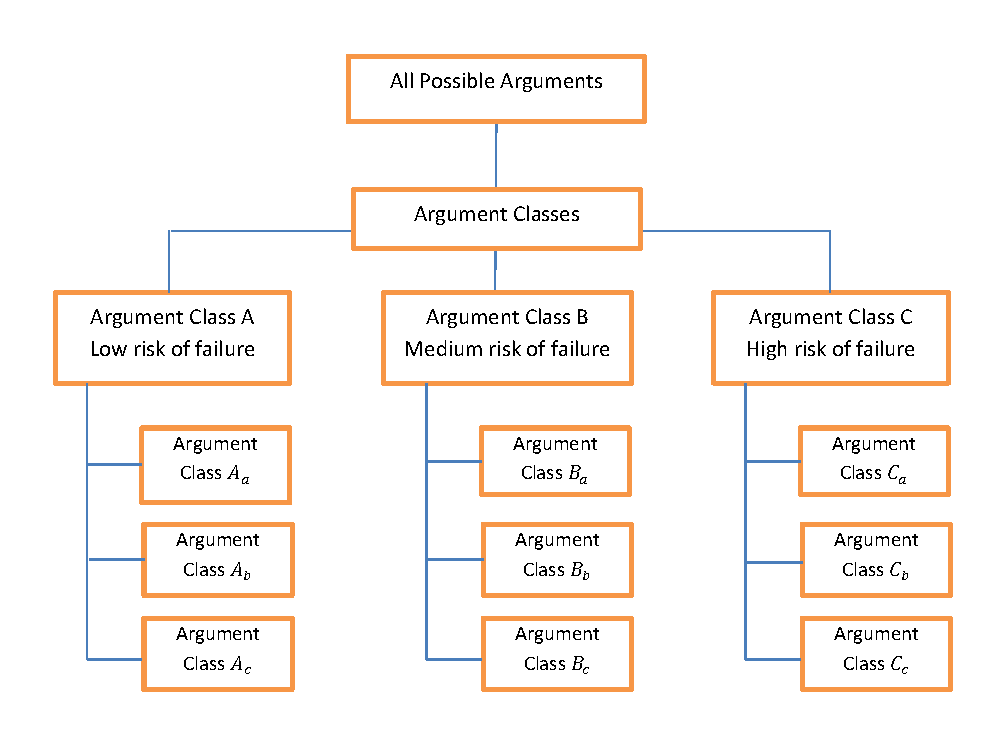
\includegraphics[width=10cm,
                height=8cm]{Figures/argumentclass.eps}\label{ClassificationFigure}
                \caption{Argument classification}
                \end{center}
\end{figure}

\textbf{Class $A$: Low risk (Highly certain arguments)}\\
Arguments of this class have equal risk, which is less than the risk of any other argument not part of that class. Formally:
\begin{equation}
Arg_i \in  A~ \text{iff}:
\begin{cases}
risk(Arg_i) = risk (Arg_j) & \forall Arg_j \in A
\\
risk(Arg_i) < risk(Arg_j)  & \forall Arg_j \notin A
\end{cases}
\end{equation}

This class is composed of three disjoint subclasses: $A_a$, $A_b$, and $A_c$, i.e., $A_a \cap A_b = A_a \cap A_c = A_b \cap A_c
=\emptyset$. Let $=_{fav}^{P_{Ag_1, Ag_2}}$ be the favorite equality relation defined as follows: for two arguments $Arg_i$ and
$Arg_j$, $Arg_i =_{fav}^{P_{Ag_1, Ag_2}} Arg_j$ iff $Arg_i \preceq_{fav}^{P_{Ag_1, Ag_2}} Arg_j$ and $Arg_j \preceq_{fav}^{P_{Ag_1, Ag_2}} Arg_i$.
The preference equality relation $=_{pref}^{Ag_1}$ is defined from $\ll_{pref}^{Ag_1}$ in the same way. $A_a$ is defined as follows:
\begin{equation}
Arg_i \in A_a~ \text{iff}:
\begin{cases}
Arg_i \in A
\\
Arg_i =_{fav}^{P_{Ag_1, Ag_2}} Arg_j & \forall Arg_j \in A_a
\\
Arg_j \preceq_{fav}^{P_{Ag_1, Ag_2}} Arg_i & \forall Arg_j \in
A-A_a
\\
Arg_i =_{pref}^{Ag_1} Arg_j & \forall Arg_j \in A_a
\\
Arg_j \prec_{pref}^{Ag_1} Arg_i & \forall Arg_j \in A-A_a
\text{~s.t.~} Arg_i =_{fav}^{P_{Ag_1, Ag_2}} Arg_j
\end{cases}
\end{equation}


This means, arguments in $A_a$ are equality favorable and preferable, more favorable than any other argument which is not
part of $A_a$, and more preferable than any other favorably equally argument.

In the sam way, the second class $A_b$ is defined as follows:
\begin{equation}
Arg_i \in A_b~ \text{iff}:
\begin{cases}
Arg_i \in A-A_a
\\
Arg_i =_{fav}^{P_{Ag_1, Ag_2}} Arg_j & \forall Arg_j \in A_b
\\
Arg_j \preceq_{fav}^{P_{Ag_1, Ag_2}} Arg_i & \forall Arg_j \in
(A-A_a)-A_b
\\
Arg_i =_{pref}^{Ag_1} Arg_j & \forall Arg_j \in A_b
\\
Arg_j \prec_{pref}^{Ag_1} Arg_i & \forall Arg_j \in (A-A_a)-A_b
\text{~s.t.~} Arg_i =_{fav}^{P_{Ag_1, Ag_2}} Arg_j
\end{cases}
\end{equation}

Finally, the third class $A_c$ is defined as follows:
\begin{equation}
A_c = (A-A_a)-A_b = A-(A_a \cup A_b)
\end{equation}



\textbf{Class $B$: Medium risk (Medium certain arguments)}\\
Arguments of this class have equal risk, which is less than the risk of any other argument not part of the union of that class and
Class $A$. Formally:
\begin{equation}
Arg_i \in B~ \text{iff}:
\begin{cases}
risk(Arg_i) = risk (Arg_j) & \forall Arg_j \in B
\\
risk(Arg_i) < risk(Arg_j) & \forall Arg_j \notin A \cup B
\end{cases}
\end{equation}

As for Class $A$, this class is composed of three disjoint subclasses: $B_a$, $B_b$, and $B_c$. $B_a$ is defined as follows:
\begin{equation}
Arg_i \in B_a~ \text{iff}:
\begin{cases}
Arg_i \in B
\\
Arg_i =_{fav}^{P_{Ag_1, Ag_2}} Arg_j & \forall Arg_j \in B_a
\\
Arg_j \preceq_{fav}^{P_{Ag_1, Ag_2}} Arg_i & \forall Arg_j \in
B-B_a
\\
Arg_i =_{pref}^{Ag_1} Arg_j & \forall Arg_j \in B_a
\\
Arg_j \prec_{pref}^{Ag_1} Arg_i & \forall Arg_j \in B-B_a
\text{~s.t.~} Arg_i =_{fav}^{P_{Ag_1, Ag_2}} Arg_j
\end{cases}
\end{equation}

%This means, arguments in $A_a$ are equally favorable and
%preferable, more favorable than any other argument which is not
%part of $A_a$, and more preferable than any other favorably
%equally argument.

In the sam way, the second class $B_b$ is defined as follows:
\begin{equation}
Arg_i \in B_b~ \text{iff}:
\begin{cases}
Arg_i \in B-B_a
\\
Arg_i =_{fav}^{P_{Ag_1, Ag_2}} Arg_j & \forall Arg_j \in B_b
\\
Arg_j \preceq_{fav}^{P_{Ag_1, Ag_2}} Arg_i & \forall Arg_j \in
(B-B_a)-B_b
\\
Arg_i =_{pref}^{Ag_1} Arg_j & \forall Arg_j \in B_b
\\
Arg_j \prec_{pref}^{Ag_1} Arg_i & \forall Arg_j \in (B-B_a)-B_b
\text{~s.t.~} Arg_i =_{fav}^{P_{Ag_1, Ag_2}} Arg_j
\end{cases}
\end{equation}

Finally, the third class $B_c$ is defined as follows:
\begin{equation}
B_c = (B-B_a)-B_b = B-(B_a \cup B_b)
\end{equation}

\textbf{Class $C$: High risk (Uncertain arguments)}\\
This class is simply defined from the two other classes where $\mathbb{A}_{C_{Ag_1, Ag_2}}$ is the set of arguments in the
context $C_{Ag_1, Ag_2}$ as follows:
\begin{equation}
C = \mathbb{A}_{C_{Ag_1, Ag_2}}-(A \cup B)
\end{equation}

The subclasses $C_a$, $C_b$, and $C_c$ are defined in the same way as the subclasses of $A$ and $B$.

The following theorem is straightforward from the above equations and Definition \ref{probabilityorderingrelation}.
\begin{theorem}
Arguments in Class $A$ have higher probability to be accepted than arguments in Class $B$ and arguments in class $B$ have higher
probability to be accepted than arguments in Class $C$.
\end{theorem}




\begin{comment}

If the argument contains formulas $\in CK$, then the $risk(Arg_i)= v1$ and in this case the argument has less risk of failure because the $CK$ has certain information (i.e., $v1$ can be equal to 0) and therefore, it has a higher chance to be accepted by the addressee. Furthermore, we distinguish three other sub-classes in case of there is more than one argument with risk of failure = $v1$, and they differ in terms of favorite and preference relations, these subclasses are as follows:\\
\textit{Class a1:} the argument is class $a1$ if it is more favorable compared to the other arguments that have the same risk of failure $v1$.\\
\textit{Class a2:} if there is more than one argument equally favorable in addition to the equality of risk failure $v1$, then we assign class $a2$ to the more preferred one, and \\
\textit{Class a3}: to the less preferred one.\\

\textbf{Class B: Arguments contain only formulas in $P_{Ag_1,Ag_2}$.}\\
If the arguments contain formulas $\in P_{Ag_1,Ag_2}$, then the $risk(Arg_i)= v2$ and in this case the risk of failure of the argument is greater than that in \textit{class A} (i.e., $v1 < v2$) because the information in $P_{Ag_1,Ag_2}$ is not certain, and therefore, the chance to be accepted by the addressee is less. As in \textit{class A}, we distinguish three other sub-classes in case of there is more than one argument with risk of failure = $v2$ and they differ in terms of favorite and preference relations, these sub-classes are as follows:\\

\textit{Class b1:} the argument is class $b1$ if it is more favorable compared to the other arguments that have the same risk of failure $v2$.\\
\textit{Class b2:} if there is more than one argument equally favorable in addition to the equality of risk failure $v2$, then we assign class $b2$ to the more preferred one, and \\
\textit{Class b3}: to the less preferred arguments.\\

\textbf{Class C: Otherwise: ``Argument contains formulas not in $CK$ and not in $P_{Ag_1,Ag_2}$".}\\

If the arguments contain formulas $\notin CK$ and $\notin
P_{Ag_1,Ag_2}$, then the $risk(Arg_i)= v3$ and in this case the
risk of failure of the argument is greater than that in
\textit{class A} and \textit{class B}
(i.e., $v1  < v2  < v3$) and consequently, the chance to be accepted by the addressee is more less than the above two classes. As in \textit{class A} and in class \textit{class B}, we distinguish three other sub-classes in case of there is more than one argument with risk of failure = $v3$ and they differ in terms of favorite and preference relations, these subclasses are as follows:\\
\textit{Class c1:} the argument is class $c1$ if it is more favorable compared to the other arguments that have the same risk of failure $v3$ .\\
\textit{Class c2:} if there is more than one argument equally favorable in addition to the equality of risk failure $v3$, then we assign class $c2$ to the more preferred one, and \\
 \textit{Class c3}: to the less preferred arguments.\\
Where $v1 < v2 < v3$ and $v1, v2, v3 \in R$.



To measure the agent's uncertainty/certainty that the selected argument will be accepted by the addressee (here we will call it the \textit{uncertainty/ceratinty degree} to distinguish it from the \textit{uncertainty index}), will use the same formulas that we used in section (~\ref{sec:type1}). Now let us present the different situations to distinguish between these two types of uncertainty.

\subsubsection{Different Cases}\label{sec:cases}
We can distinguish three different cases that make the difference between two types of the agent's uncertainty clear.\\

\textbf{Case 1: If there is only one possible argument}.\\
If the agent has just one possible argument, then the probability of that argument will be at its maximum value (i.e., equal to one to satisfy the probability condition $\Sigma_{m_{j}^{i} \in PA_{i}} P(m_{j}^{i}=1))$ and the uncertainty degree will be at its minimum value (i.e., equal to zero, based on proposition~\ref{proposition1}). In this case the \textit{uncertainty degree} is equal to the \textit{uncertainty index} and it does not represent the agent's uncertainty that the selected move will be accepted by the addressee, it rather represents the agent's uncertainty about selecting the right argument at that step, regardless it will be accepted by the addressee agent or not, because the available argument can be any of the above classes, and therefore, if the class of the argument is $C$ for instance, then the chance for this argument to be accepted is very weak and this contradicts the high probability assigned to this argument (equal to one). However, this is not applicable for all classes, for example if the argument is class $A$, then there is a high chance to be accepted, so the high probability assigned matches the low uncertainty we achieved and this a special case of \textit{case 1}.

\begin{proposition} \label{proposition3}
In negotiation dialogue games, at each dialogue step the uncertainty degree is equal to the uncertainty index, and it represents the agent's uncertainty about selecting the right argument as well as the agent's uncertainty about the selected argument to be accepted by the addressee and it will be at it's minimum value iff at that step there is only one possible argument and it has class A.
\end{proposition}

\textbf{proof}\\
From proposition~\ref{proposition1}, it's clear that the uncertainty of selecting the right move will be at its minimum
value ``0" iff there is only one possible argument, and if the class of this argument is A, then the risk of failure is at its
minimum value too, which means the uncertainty about the argument to be accepted is at its minimum value ``0". So the uncertainty of
selecting the right argument ``certainty index" and the uncertainty about the argument to be accepted by the addressee
``certainty degree" is the same.  ~~~~~~~~~$\blacksquare$


\begin{proposition} \label{proposition4}
In negotiation dialogue games, at each dialogue step if there is only one possible argument, the uncertainty degree is equal to the uncertainty index and it just represents the agent's uncertainty about selecting the right argument iff that argument is not class A.
\end{proposition}

\textbf{proof}\\
If there is only one possible argument, the uncertainty will be at its minimum value ``0" ~\ref{proposition1}. Now, if the available
argument is not class A, then the risk of failure will be greeter than V1. In this case we can not consider the uncertainty value
``0" as an indicator for the move to be accepted by the addressee, rather, we consider it as an index of selecting the right argument
since there is no other choice. ~~~~~~~~~$\blacksquare$

\textbf{Case 2: If there is more than one possible argument with the same class}.\\
If all possible arguments have the same class then they will be equally probably to be selected and the uncertainty will be at its maximum value (i.e., equal to one, following proposition 2), and again as in case 1, it does not always represent the uncertainty about the selected argument to be accepted or refused by the addressee, because the possible arguments might have a high risk of failure (e.g. in class c), in this case it represents the agent's uncertainty about the argument to be accepted. In the other hand, if all arguments have class A, for example, which means a very low risk of failure, then the uncertainty does not represent the uncertainty that the argument will be accepted, it rather represents the uncertainty about selecting the right move.

\begin{proposition} \label{proposition5}
In negotiation dialogue games, if all possible arguments at certain dialogue step have the same class, then the uncertainty of the selected argument is at its maximum value, and it represents only the agent's uncertainty about selecting the right argument, except if the arguments are class C.
\end{proposition}

\textbf{proof}\\
If all possible arguments have the same class, then they will have same probability value which leads to maximum value of uncertainty
``1" see~\ref{proposition2}. If the arguments have class A, then the risk of failure will be at its minimum value ``0", and in this
case the low risk of failure contradict the high uncertainty for the argument to be accepted. So we can not consider this high
uncertainty as an indicator of accepting. ~~~~~~~~~$\blacksquare$


\textbf{Case 3: If there is more than one argument with different classes}.\\
In this case, the assignment of the probability will be based on the class of the argument, and following the argument selection mechanism, the agent will select the higher argument class, so the uncertainty in this case represents the agent's uncertainty that the selected argument will accepted by the addressee. This will enhance the performance of the agent towards achieving the dialogue goal.\\
The different cases that show the argument class and the associated type of uncertainty are summarized in    Table~\ref{Table4}.

\begin{table}[tbp]
\centering \caption{Argument classes vs. Uncertainty types} \label{Table4}
\begin{tabular}{||c|c|c|c||}\hline\hline
\multicolumn{4}{||c||}{\textbf{Number of possible arguments}} \\
\hline\hline
One possible argument & Uncertainty Type  & More than one possible argument & Uncertainty Type \\
\hline
Class A               & Type  I / Type II & Same class =  Class A   & Type  I \\ \hline
Class B               & Type  I           & Same class =  Class B   & Type  I \\ \hline
Class C               & Type  I           & Same class =  Class C   & Type  I \\ \hline
                      &                   & Different classes       &Type  I / Type  II\\
\hline
\end{tabular}
\end{table}

\end{comment}


